\documentclass[runningheads]{llncs}
% PROVISIONAL: official Springer LLNCS class v2.26 (CTAN mirror of Springer's llncs package). Generated by build_main.py.
% (no T1 fontenc: avoids bitmap font generation)
\usepackage{graphicx}
\usepackage{booktabs}
\usepackage{amsmath,amssymb}
\usepackage{algorithm}
\usepackage{algpseudocode}
\usepackage{url}
\usepackage{array}
\setcounter{topnumber}{3}\setcounter{totalnumber}{5}\renewcommand{\topfraction}{0.9}\renewcommand{\bottomfraction}{0.8}\renewcommand{\textfraction}{0.1}\renewcommand{\floatpagefraction}{0.75}
\begin{document}
\title{Does Dimensionality Reduction Help Classical Intrusion Detection? Original Features versus PCA and Kernel PCA on a Class-Stratified CIC-IDS2017 Sample}
\titlerunning{Dimensionality Reduction for Classical Intrusion Detection}
\author{[AUTHOR NAME 1 -- TO BE FILLED]\inst{1} \and [AUTHOR NAME 2 -- TO BE FILLED]\inst{1}}
\authorrunning{[A. Author et al. -- TO BE FILLED]}
\institute{[DEPARTMENT, INSTITUTION, CITY, COUNTRY -- TO BE FILLED]\\ \email{[EMAIL -- TO BE FILLED]}}
\maketitle
\begin{abstract}
Kernel principal component analysis is often paired with classical classifiers for network intrusion detection, but gains are usually reported as single-split accuracy without a no-reduction baseline. This study compares the 78 original flow features with principal component analysis and kernel principal component analysis (linear, radial basis function and cosine kernels; 5 to 30 components) across five classifiers. The data are a 6,000-record sample drawn from all eight CIC-IDS2017 files after exact-duplicate removal. The sample is class-stratified, with at least 100 records per class, and does not preserve natural traffic prevalence. Imputation, scaling and reduction are fitted on training folds only. Evaluation combines repeated stratified cross-validation, nested cross-validation, a small nested hyper-parameter search, two row-order robustness checks serving as a proxy for chronology (the files contain no timestamps), and a runtime and memory benchmark. A random forest on the original features achieved the highest observed macro-averaged F1 score, 0.901 $\pm$ 0.020 (accuracy 0.972 $\pm$ 0.004; nested estimate 0.900 $\pm$ 0.022). Accuracy hides weak detection of two web attack classes (F1 0.53 and 0.59). Original features outperformed both reductions for the decision tree and random forest and matched them for logistic regression and $k$-nearest neighbors; only the support vector machine benefited from reduction, and its advantage fell from 0.076 to 0.021 after tuning. Kernel analysis took more than 200 times longer to fit than principal component analysis and about 37 times more traced memory. The findings are limited to one sample of one dataset.

\keywords{Network intrusion detection \and CIC-IDS2017 \and Kernel PCA \and Dimensionality reduction \and Class imbalance \and Machine learning.}
\vspace{2pt}\noindent\textit{Code and results:} [REPOSITORY URL / ARCHIVE DOI -- TO BE FILLED BY THE AUTHORS]
\end{abstract}

\section{Introduction}
Machine-learning network intrusion detection systems (NIDS) are commonly developed and compared on public flow datasets \cite{ring2019}, of which CIC-IDS2017 \cite{sharafaldin2018} is widely used. Its flow records, as distributed in the MachineLearningCVE files, carry 78 numeric features, which motivates dimensionality reduction as a way to cut training cost and possibly improve generalization. Linear PCA and auto-encoders have been applied to CIC-IDS2017 \cite{abdulhammed2019}, and Kernel PCA (KPCA) \cite{scholkopf1998}, which performs PCA in an implicit nonlinear feature space, has been combined with SVMs for intrusion detection \cite{kuang2014}.

Three methodological issues make such comparisons hard to interpret. First, CIC-IDS2017 is class-imbalanced and, in its original form, contains labelling and flow-construction problems \cite{engelen2021,panigrahi2018}, so accuracy can be dominated by the benign majority. Second, pitfalls in security-oriented machine learning can lead to over-optimistic performance estimates \cite{arp2022}. Third, a no-reduction baseline is the necessary control for any claim that reduction helps; without it, a benefit is assumed rather than measured.

\textbf{Research questions.} We ask: \textbf{RQ1} how does reduction affect multi-class detection performance; \textbf{RQ2} does KPCA beat the original space or conventional PCA; \textbf{RQ3} how do kernel, component count and classifier interact; \textbf{RQ4} what does the reduction cost in time and memory; \textbf{RQ5} how stable are the conclusions under repeated, class-aware validation, nested selection, tuning, row-order splits (a proxy for chronology) and smaller training sets.

\textbf{Contributions.} (i) A reproducible comparison of original features, PCA and three KPCA kernels over five classical classifiers on a raw-data-derived sample drawn after exact same-label duplicate removal, with fold-wise fitting, a majority-class baseline, a nested-CV check of selection optimism and a small nested hyper-parameter search. (ii) A class-aware analysis showing how much accuracy overstates detection quality. (iii) Paired statistical tests with an explicit independence caveat, and two row-order robustness checks (proxy chronology). (iv) A runtime and memory measurement of KPCA against PCA. We do not propose a new algorithm; code and results are described in the Data and Code Availability section.

\section{Related Work}
We surveyed fifteen studies. Table~\ref{tab:lit} lists five recent (2025) studies with algorithm, dataset and result \emph{as stated by their authors}; ten more, on the dataset, its problems, dimensionality reduction and evaluation practice, are discussed below. Their numbers use different datasets, splits and metrics and are not a ranking.


\textit{Dataset and its problems.} Ring et al.\ review public network-intrusion datasets and define 15 properties for judging which evaluation settings each dataset fits \cite{ring2019}. CIC-IDS2017 was introduced by Sharafaldin et al.\ \cite{sharafaldin2018}. Engelen et al.\ report problems in it: ``TCP appendix'' artefact flows (about a quarter of all flows), attack attempts labelled as attacks although they contain no malicious payload, and feature-extraction flaws that enable shortcut learning; they released a corrected version \cite{engelen2021}. Panigrahi and Borah likewise describe shortcomings and propose a combined dataset \cite{panigrahi2018}. We use the \emph{original} labelled flows, so absolute scores may partly reflect such artefacts.

\textit{Dimensionality reduction and feature selection.} Abdulhammed et al.\ apply an auto-encoder and PCA to CIC-IDS2017 (81 to 10 dimensions) and report about 99.6\,\% accuracy \cite{abdulhammed2019}; Kuang et al.\ combine KPCA, an SVM and a genetic algorithm \cite{kuang2014}. Abdel-Rahman et al.\ state that a feature-importance-guided autoencoder outperforms PCA on three datasets including CIC-IDS2017 \cite{abdelrahman2026}. Chavan and Alone report ``high accuracy'' for a random forest on CIC-IDS 2017 without a figure or split in the abstract \cite{chavan2025}, and Patil et al.\ include PCA among their reduction methods \cite{patil2025}. Most report accuracy on one split; none that we read pairs a no-reduction baseline, per-class analysis and fold-wise fitting across PCA and several KPCA kernels.

\textit{Evaluation practice.} Arp et al.\ describe pitfalls in machine learning for security that can lead to unrealistic performance \cite{arp2022}, and Apruzzese et al.\ propose cross-evaluating ML-based NIDS across datasets \cite{apruzzese2022}. Following them we fit every data-dependent step on training folds only, report class-aware metrics beside accuracy, include trivial and no-reduction baselines, and state what our sample cannot show. This is not a systematic survey. IEEE Xplore pages could not be retrieved from our environment, so the studies above come from open publisher and preprint pages.

\begin{table}[htbp]
\caption{Recent studies (2025) and this work. Results are quoted from each source and are not directly comparable (different datasets, sampling, splits and metrics).}\label{tab:lit}
\centering\scriptsize
\renewcommand{\arraystretch}{1.15}
\begin{tabular}{@{}>{\raggedright\arraybackslash}p{2.3cm}>{\raggedright\arraybackslash}p{3.3cm}>{\raggedright\arraybackslash}p{2.4cm}>{\raggedright\arraybackslash}p{1.7cm}>{\raggedright\arraybackslash}p{1.7cm}@{}}
\toprule
Author (year) & Title & Algorithm & Dataset & Reported result \\
\midrule
Waghmode et al.\ \cite{waghmode2025} (2025) & Intrusion detection system based on machine learning using least square support vector machine & Quantum-inspired LS-SVM with exhaustive feature selection & NSL-KDD, CIC-IDS-2017, UNSW-NB15 & Accuracy 99.5\,\% on CIC-IDS-2017 \\
Patil et al.\ \cite{patil2025} (2025) & Optimizing network intrusion detection systems through ensemble learning and feature selection using the CIC-IDS2017 dataset & Bagging and boosting ensembles; information gain, chi-square, PCA (20 features) & CIC-IDS2017, stratified 70/30 split & Accuracy 99.98\,\% (Extra Trees, 24 features); 99.58--99.96\,\% with PCA \\
Abdelaziz et al.\ \cite{abdelaziz2025} (2025) & Enhancing network threat detection with random forest-based NIDS and permutation feature importance & Random forest, permutation importance, undersampling; repeated stratified 5-fold CV & CIC-IDS2017 & Weighted-F1 99.8\,\%, macro-F1 93.31\,\% (26 features) \\
Xu and Liu \cite{xu2025} (2025) & Robust anomaly detection in network traffic: evaluating machine learning models on CICIDS2017 & MLP, 1D-CNN, one-class SVM, LOF & CICIDS2017 & Accuracy 97.75\,\% (MLP, overall test set) \\
Emirmahmuto\u{g}lu and Atay \cite{emirmahmutoglu2025} (2025) & A feature selection-driven machine learning framework for anomaly-based intrusion detection systems & PSO/FPA/DE feature selection; LR, DT, RF, k-NN and others & KDD CUP 99, NSL-KDD, UNSW-NB15, CSE-CIC-IDS2018 & Accuracy 99.9965\,\% on CSE-CIC-IDS2018 (FPA, RF) \\
\midrule
\textbf{This work} (2026) & (this paper) & Original features vs PCA vs linear/RBF/cosine KPCA; LR, k-NN, SVM, DT, RF & CIC-IDS2017, 6,000-record class-stratified sample & RF (original): accuracy 97.2\,\%, macro-F1 90.1\,\% \\
\bottomrule
\end{tabular}
\end{table}

\section{Dataset and Preprocessing}\label{sec:data}
\textbf{Data.} We use the eight daily CIC-IDS2017 \texttt{MachineLearningCVE} files: 2{,}830{,}743 flows, 78 numeric features, 15 labels (counts computed from the files; no provider checksum was available). There is no timestamp column. Rows with missing or infinite values are 0.2\,\% or less of each file (inf $\to$ NaN) and were not imputed before sampling. Eight features are constant in every file and were kept to match the 78-feature definition of earlier work.

\textbf{Duplicates.} 308{,}381 flows (10.9\,\%) are exact duplicates (identical on all 78 features and the label) of another flow and were removed before sampling, because identical flows in training and test folds inflate scores. Feature-identical flows with \emph{different} labels were not removed: 698 such conflicting-label groups remain in the 2.52\,M pool. None of them fell into the 6{,}000-record sample: it contains no two records with identical feature vectors, with the same or with different labels. Duplication is uneven: removal took 43\,\% of PortScan flows (158{,}930 to 90{,}819) and 25\,\% of DoS Hulk flows, versus 7.8\,\% of benign flows.

\textbf{Sample.} Exact KPCA needs an $n\times n$ kernel matrix, so we draw a stratified random sample of 6{,}000 records from the de-duplicated pool of 2{,}522{,}362 flows (seed 0): each class contributes at least 100 records (all of them if fewer exist) and the rest is allocated proportionally to pool prevalence. Heartbleed (11), SQL injection (21) and Infiltration (36) are therefore complete but tiny; the floor over-represents attack classes relative to real traffic (benign: 67.2\,\% of the sample versus 83\,\% of the pool). Sampling uses only labels and random numbers; \emph{no imputation or scaling statistic is computed before the split}. Only two feature cells in the sample are missing; they are imputed with training-fold means inside each fold. The sample also stores each record's source file (day) and original row position, used for the row-order checks below.



\section{Methodology}\label{sec:method}
\textbf{Pipeline.} Fig.~\ref{fig:pipe} shows the protocol. Within each training fold we fit a mean imputer and a standard scaler, then the dimensionality reducer; test folds are only transformed. Feature spaces are: \emph{original} (78 standardised features); \emph{PCA}; and \emph{KPCA} with linear, RBF (scikit-learn default $\gamma=1/78$) and cosine kernels \cite{scholkopf1998}, each with $n\in\{5,10,15,20,30\}$ components. The reducer is fitted once per fold and shared by all classifiers, which is equivalent to fitting it inside each pipeline because it is deterministic (unit-tested).

\begin{figure}[htbp]\centering
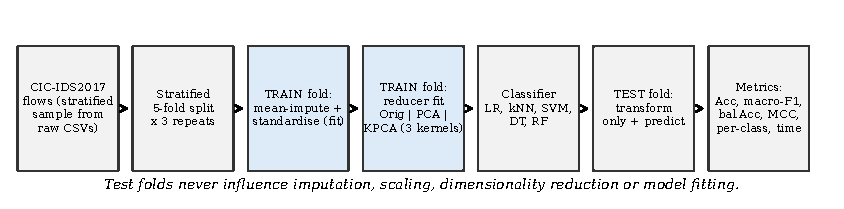
\includegraphics[width=\textwidth]{figures/fig1_pipeline.pdf}
\caption{Experimental pipeline. All data-dependent preprocessing and reduction is fitted on the training fold only.}\label{fig:pipe}
\end{figure}

\textbf{Algorithm and formulas.} Algorithm~\ref{alg:cv} summarises one evaluation of a feature space and classifier. Features are standardised as $z_j=(x_j-\mu_j)/\sigma_j$ with $\mu_j,\sigma_j$ from the training fold. PCA projects onto the leading eigenvectors $\mathbf{v}_k$ of the training covariance matrix $\mathbf{C}=\frac{1}{n}\mathbf{Z}^{\top}\mathbf{Z}$. KPCA uses the kernel matrix $K_{ij}=k(\mathbf{z}_i,\mathbf{z}_j)$ with
\begin{equation}
k_{\mathrm{lin}}=\mathbf{z}^{\top}\mathbf{z}',\qquad k_{\mathrm{rbf}}=\exp(-\gamma\lVert\mathbf{z}-\mathbf{z}'\rVert^{2}),\ \gamma=\tfrac{1}{78},\qquad k_{\cos}=\frac{\mathbf{z}^{\top}\mathbf{z}'}{\lVert\mathbf{z}\rVert\,\lVert\mathbf{z}'\rVert},
\end{equation}
centred as $\tilde{K}=K-\mathbf{1}_nK-K\mathbf{1}_n+\mathbf{1}_nK\mathbf{1}_n$; a sample is projected to $\tilde{K}\boldsymbol{\alpha}_k/\sqrt{\lambda_k}$ for the leading eigenpairs $(\lambda_k,\boldsymbol{\alpha}_k)$. With per-class precision $P_c$ and recall $R_c$, the primary metric is
\begin{equation}
F1_c=\frac{2P_cR_c}{P_c+R_c},\qquad \text{macro-F1}=\frac{1}{C}\sum_{c=1}^{C}F1_c,\ \ C=15,
\end{equation}
and balanced accuracy equals macro-recall. The multi-class MCC from the confusion matrix $\mathbf{M}$ with $s$ samples, $t_k$ true and $p_k$ predicted counts of class $k$, and $c=\sum_k M_{kk}$ correct predictions is
\begin{equation}
\mathrm{MCC}=\frac{c\,s-\sum_k p_kt_k}{\sqrt{s^{2}-\sum_k p_k^{2}}\,\sqrt{s^{2}-\sum_k t_k^{2}}}.
\end{equation}

\begin{algorithm}[t]
\caption{Fold-wise evaluation of one feature space $S$ and classifier $f$}\label{alg:cv}
\begin{algorithmic}[1]
\Require sample $(X,y)$ of 6,000 records; space $S\in\{$original, PCA, KPCA$(k,n)\}$; classifier $f$; 3 repeats of stratified 5-fold CV (seed 42)
\Ensure mean and standard deviation of accuracy, macro-F1, MCC and cost over 15 folds
\For{each repeat $r$ and fold $(\mathrm{tr},\mathrm{te})$}
  \State fit mean imputer and standard scaler on $X_{\mathrm{tr}}$; transform $X_{\mathrm{tr}}$ and $X_{\mathrm{te}}$
  \If{$S\neq$ original}
    \State fit reducer $T_S$ ($n$ components) on the scaled $X_{\mathrm{tr}}$ only
    \State $Z_{\mathrm{tr}}\gets T_S(X_{\mathrm{tr}})$;\ $Z_{\mathrm{te}}\gets T_S(X_{\mathrm{te}})$
  \Else
    \State $Z_{\mathrm{tr}}\gets X_{\mathrm{tr}}$;\ $Z_{\mathrm{te}}\gets X_{\mathrm{te}}$
  \EndIf
  \State fit $f$ on $(Z_{\mathrm{tr}},y_{\mathrm{tr}})$;\ predict $\hat{y}$ on $Z_{\mathrm{te}}$; record metrics and fit time
\EndFor
\State \Return mean $\pm$ std over the 15 folds (nested selection repeats this inside each outer training set with 3 inner folds)
\end{algorithmic}
\end{algorithm}

\textbf{Classifiers.} Logistic regression (L2, lbfgs), $k$-NN with $k=5$ \cite{cover1967}, an SVM with RBF kernel, $C=1$ and $\gamma$=``scale'' \cite{cortes1995}, a decision tree with entropy criterion \cite{quinlan1986}, and a random forest with 100 trees \cite{breiman2001}, using scikit-learn \cite{pedregosa2011}. The main grid uses these fixed default settings; a separate nested search (below) tests whether tuning changes the conclusions. Each classifier except $k$-NN is also run with \texttt{class\_weight=balanced}. A majority-class classifier is the trivial baseline. Resampling (e.g.\ SMOTE) is not used: Heartbleed has only 8--9 training records per fold, too few for meaningful synthetic interpolation.

\textbf{Validation.} Repeated stratified 5-fold cross-validation, 3 repeats (15 folds), seed 42; every method sees identical folds, giving paired observations. Test folds hold about 2 Heartbleed and 4 SQL-injection records, so per-class estimates for these classes are noisy; we report means and standard deviations over the 15 folds.

\textbf{Nested cross-validation for selection.} Choosing the best of 189 configurations (21 feature spaces $\times$ 9 classifier/weighting variants) on the scoring folds is optimistic. On the \emph{same} 15 outer folds, a stratified 3-fold inner cross-validation inside each outer training set (4{,}800 records) scores every configuration by macro-F1, the best is selected, and only it is scored on the untouched outer test fold. We apply this to (A) the global selection and, per classifier, to (C) the best \emph{reduced} space and weighting versus (D) the original space with weighting chosen the same way; all steps are refitted on every inner split.

\textbf{Nested hyper-parameter search.} For $k$-NN, SVM and random forest on four spaces (original, PCA-30, KPCA-cosine-30, KPCA-RBF-30), a 3-fold inner cross-validation inside each of the first five outer folds selects from small grids: $k\in\{3,5,7,11\}$; SVM $C\in\{0.1,1,10\}$, $\gamma\in\{\text{scale},0.01,0.1\}$, class weight none/balanced; random forest 100/200 trees, depth none/10/20, class weight none/balanced. The RBF width of the KPCA reducer itself is not tuned.

\textbf{Row-order robustness checks (proxy chronology).} The raw files have no timestamps; attack flows occur in contiguous row blocks, so we \emph{assume}, without proof, that row order follows capture time. (i) \emph{Head/tail}: the first 70\,\% of each file's rows train, the last 30\,\% test. (ii) \emph{Blocked CV}: each file is cut into five contiguous blocks, each held out in turn. Only classes present in both training and test are scored, and a random split of the same rows on the same classes is the comparator.

\textbf{Metrics.} Accuracy; macro-precision, macro-recall and macro-F1; weighted-F1; balanced accuracy; and the multi-class Matthews correlation coefficient (MCC) as implemented in scikit-learn (Chicco and Jurman argue for MCC in the binary case \cite{chicco2020}). \textbf{Macro-F1 is the primary model-selection criterion}, chosen before the runs because it weights all 15 classes equally. Per-class results and the confusion matrix use pooled out-of-fold predictions of the first repeat.

\textbf{Statistics.} Per classifier we compare feature spaces at matched $n=10$ with two-sided Wilcoxon signed-rank tests on the 15 paired macro-F1 values, Holm-corrected over 30 comparisons, with the rank-biserial correlation $r$ as effect size, and Friedman omnibus tests, following the non-parametric procedures of Dem\v{s}ar \cite{demsar2006} (written for several data sets; here the blocks are folds of one sample). Because folds share training data, the 15 differences are positively correlated and naive $p$-values are too liberal \cite{nadeau2003}; we do not apply the Nadeau--Bengio correction and use the tests for screening, not as proof. Comparisons against each classifier's \emph{best} reduced space are selected on the same folds, which favours the reduced space; the nested analysis removes that bias.

\textbf{Cost.} A serial benchmark (no parallel workers) records training and inference time (median of 5 repetitions, one fold split) and peak memory from Python's \texttt{tracemalloc}, measured in a separate pass. Native allocations inside compiled code are not traced, so memory figures are lower bounds most reliable for comparing reducers.

\textbf{Setup.} A 2-vCPU, 7\,GB VM (Python 3.13, scikit-learn 1.9) ran the main grid (2{,}850 fits, about 28 min), nested CV (about 64 min) and tuning (about 16 min); cost timings come from a separate serial benchmark (4{,}800 training, 1{,}200 test records).

\section{Results}
\subsection{Original-feature baseline and the cost of reading accuracy alone}
Predicting the majority class gives accuracy 0.672 but macro-F1 0.054 and MCC 0.000. The random forest on original features reaches accuracy $0.972\pm0.004$ but macro-F1 $0.901\pm0.020$ (weighted-F1 0.971, balanced accuracy 0.883, MCC $0.948\pm0.008$): accuracy exceeds macro-F1 by 0.071, and the gap comes from a few classes. Per class (Table~\ref{tab:perclass}), ten of the 15 classes, including benign, DDoS, the four DoS families, both Patator brute-force classes, PortScan and Heartbleed, have F1 $\ge$ 0.96. The weak points are web brute force (F1 0.53) and web XSS (0.59), which are largely mistaken for each other (48 of 103 brute-force records are predicted as XSS and 35 of 101 XSS records as brute force), then bot (0.87; recall 0.82), infiltration (0.875; recall 0.78, 36 records) and SQL injection (0.84; 21 records). Engelen et al.\ find that most web brute-force and XSS flows carry no payload in the forward direction \cite{engelen2021}, which may explain why they are hard to separate. These are the weak points that accuracy hides (Table~\ref{tab:perclass}).

\begin{table}[htbp]
\caption{Per-class results of the selected model (RF, original features), pooled out-of-fold predictions, first repeat.}\label{tab:perclass}
\centering\scriptsize
\begin{tabular}{lrrrr}
\toprule
Class & Precision & Recall & F1 & Support \\
\midrule
BENIGN & 0.984 & 0.996 & 0.990 & 4034 \\
Bot & 0.924 & 0.817 & 0.867 & 104 \\
DDoS & 0.997 & 0.997 & 0.997 & 340 \\
DoS GoldenEye & 0.975 & 0.966 & 0.970 & 119 \\
DoS Hulk & 0.998 & 0.979 & 0.988 & 424 \\
DoS Slowhttptest & 0.955 & 0.973 & 0.964 & 110 \\
DoS slowloris & 1.000 & 0.927 & 0.962 & 110 \\
FTP-Patator & 1.000 & 1.000 & 1.000 & 111 \\
Heartbleed & 1.000 & 1.000 & 1.000 & 11 \\
Infiltration & 1.000 & 0.778 & 0.875 & 36 \\
PortScan & 0.989 & 0.981 & 0.985 & 270 \\
SSH-Patator & 1.000 & 0.943 & 0.971 & 106 \\
Web Brute Force & 0.581 & 0.485 & 0.529 & 103 \\
Web Sql Injection & 0.941 & 0.762 & 0.842 & 21 \\
Web XSS & 0.558 & 0.624 & 0.589 & 101 \\
\bottomrule
\end{tabular}

\end{table}





\subsection{Original space versus PCA versus Kernel PCA}
Table~\ref{tab:n10} and Fig.~\ref{fig:all} compare spaces at $n=10$. Of the 30 Holm-corrected comparisons, 23 were significant. The original space was significantly better than PCA-10 for logistic regression, SVM, decision tree and random forest, and than RBF-10 and cosine-10 for all five classifiers; for $k$-NN it was indistinguishable from PCA-10 ($\Delta$ macro-F1 $-0.001$). Among the reduced spaces, RBF-KPCA was significantly worse than PCA for LR, $k$-NN, DT and RF, but \emph{better} than PCA for the SVM; cosine KPCA was significantly better than PCA for the SVM ($+0.120$), worse for LR, $k$-NN and DT, and not different for RF. Linear KPCA and PCA did not differ significantly for any classifier. The Friedman omnibus tests (spaces at $n=10$ within each classifier; classifiers within each space) were all significant (statistics 46.8--57.6 and 51.9--58.1, Holm-adjusted $p\le 2.7\times10^{-9}$ in every case), but they inherit the fold-dependence caveat above and serve only as screening. Against each classifier's \emph{best} reduced space (table in the repository), original features were clearly better for DT ($+0.070$) and RF ($+0.056$; $p_\mathrm{Holm}=0.0003$, better in all 15 folds); for logistic regression the best reduced space (PCA, 30 components) came within 0.004 ($p_\mathrm{Holm}=0.021$, a significant but negligible gap); $k$-NN showed no difference; and the SVM was the single clear case where reduction helped: cosine KPCA with 30 components raised macro-F1 from 0.675 to 0.746 ($p_\mathrm{Holm}=0.0003$, better in all 15 folds). That family of comparisons is selected on the same folds and therefore optimistic. The SVM gain needs many components: cosine KPCA reaches 0.605 at 10 components (below the original 0.675) and 0.746 at 30.

\begin{table}[htbp]
\caption{Accuracy / macro-F1 ($\pm$ std over 15 folds) at 10 components (original = 78 features), standard class weights.}\label{tab:n10}
\centering\scriptsize
\resizebox{\textwidth}{!}{\begin{tabular}{lccccc}
\toprule
Space & LR & KNN & SVM & DT & RF \\
\midrule
Original (78) & 0.924 / 0.736$\pm$0.022 & 0.934 / 0.800$\pm$0.024 & 0.906 / 0.675$\pm$0.017 & 0.964 / 0.881$\pm$0.021 & 0.972 / 0.901$\pm$0.020 \\
PCA-10 & 0.842 / 0.506$\pm$0.018 & 0.932 / 0.802$\pm$0.023 & 0.842 / 0.485$\pm$0.024 & 0.941 / 0.805$\pm$0.025 & 0.956 / 0.834$\pm$0.022 \\
KPCA-lin-10 & 0.842 / 0.507$\pm$0.017 & 0.932 / 0.802$\pm$0.023 & 0.842 / 0.485$\pm$0.024 & 0.942 / 0.806$\pm$0.024 & 0.957 / 0.836$\pm$0.019 \\
KPCA-RBF-10 & 0.805 / 0.306$\pm$0.015 & 0.918 / 0.757$\pm$0.029 & 0.880 / 0.525$\pm$0.016 & 0.920 / 0.755$\pm$0.037 & 0.937 / 0.790$\pm$0.037 \\
KPCA-cos-10 & 0.852 / 0.462$\pm$0.012 & 0.926 / 0.783$\pm$0.028 & 0.904 / 0.605$\pm$0.018 & 0.928 / 0.786$\pm$0.027 & 0.944 / 0.821$\pm$0.029 \\
\bottomrule
\end{tabular}
}
\end{table}



\subsection{All executions in one chart}
Fig.~\ref{fig:all} places every classifier and feature space at 10 components in a single chart (25 executions, macro-F1, mean $\pm$ std over 15 folds). Within each classifier group the black bar is the original space; only for the SVM does a reduced space (cosine KPCA) exceed it, and the tree-based classifiers lead overall.

\begin{figure}[htbp]\centering
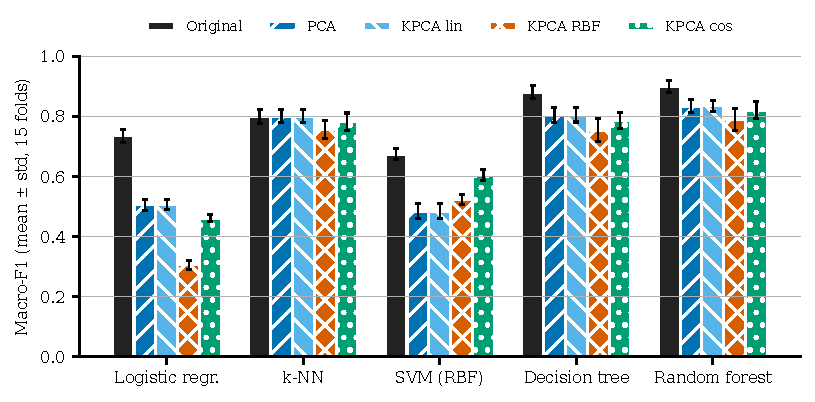
\includegraphics[width=0.9\textwidth]{figures/fig10_all_executions.pdf}
\caption{Macro-F1 of all classifier $\times$ feature-space executions at 10 components (mean $\pm$ std over 15 folds; standard class weights; axis starts at zero).}\label{fig:all}
\end{figure}

\subsection{Selection optimism: nested cross-validation}\label{sec:results-nested}
Selecting the best of 189 configurations on the scoring folds is optimistic, so selection was repeated inside a nested cross-validation (Section~\ref{sec:method}). The configuration chosen on inner folds reached macro-F1 $0.900\pm0.022$ (accuracy 0.972, MCC 0.947) on the outer folds against 0.901 for the same-CV maximum: an optimism of about 0.001. The inner folds chose an original-feature configuration in all 15 outer folds (random forest 11 times, decision tree 4). Original features were clearly better than the inner-selected best reduced space for DT ($+0.093$) and RF ($+0.062$), practically equal for logistic regression ($+0.004$, unadjusted $p=0.010$, far below the fold standard deviation of 0.022) and $k$-NN ($+0.002$), and worse for the SVM ($-0.060$; cosine KPCA-30 chosen in all 15 folds). The $p$-values are unadjusted Wilcoxon tests over 15 outer folds that share training data.



\subsection{Effect of hyper-parameter tuning}
Table~\ref{tab:tuning} reports the nested search (five outer folds). Tuning left the random forest unchanged (original 0.901 default, 0.899 tuned; best reduced 0.842 versus 0.839). For $k$-NN, tuning gave $+0.007$ on original features; the best reduced space was cosine KPCA-30 under defaults (gap 0.000) and PCA-30 after tuning (0.810 versus 0.808, gap $-0.002$; default gap in PCA-30: $+0.003$), always far below fold variation. The SVM changed most: tuned macro-F1 rose from 0.668 to 0.791 on original features and from 0.745 to 0.812 with cosine KPCA-30, so the reduced-space advantage shrank from 0.076 to 0.021. Five folds cannot establish a 0.021 difference, and the selected values sit on grid edges (SVM $C=10$ and $k$-NN $k=3$ in all 20 selections), so we treat the SVM advantage of KPCA as a property of the default RBF-SVM that largely disappears with tuning, not as a robust benefit of KPCA.

\begin{table}[htbp]
\caption{Nested hyper-parameter search: mean macro-F1 over five outer folds. For each setting (default, tuned) the best reduced space among PCA-30, KPCA-cos-30 and KPCA-RBF-30 is chosen by that setting\textquoteright s own score; $\Delta$ = original $-$ reduced (negative: reduction better). K-cos-30 = KPCA, cosine kernel, 30 components. The last column gives the default-setting gap measured in the tuned-best reduced space.}\label{tab:tuning}
\centering\scriptsize
\resizebox{\textwidth}{!}{\begin{tabular}{lccrccrr}
\toprule
 & \multicolumn{3}{c}{Default settings} & \multicolumn{3}{c}{Tuned (nested search)} & \\
\cmidrule(lr){2-4}\cmidrule(lr){5-7}
Clf & Orig. & Best reduced & $\Delta$ & Orig.  & Best reduced  & $\Delta$  & $\Delta$ def., tuned-best space \\
\midrule
KNN & 0.801 & 0.801 (K-cos-30) & +0.000 & 0.808 & 0.810 (PCA-30) & -0.002 & +0.003 \\
SVM & 0.668 & 0.745 (K-cos-30) & -0.076 & 0.791 & 0.812 (K-cos-30) & -0.021 & -0.076 \\
RF & 0.901 & 0.842 (PCA-30) & +0.059 & 0.899 & 0.839 (PCA-30) & +0.060 & +0.059 \\
\bottomrule
\end{tabular}
}
\end{table}

\subsection{Row-order robustness (proxy chronology)}
In the head/tail split 4{,}199 records train and 1{,}769 test (32 test records of unseen classes were dropped); only seven of the 15 classes occur in both parts, and infiltration has four test records. The random forest on original features scored 0.838 versus 0.948 for a random split of the same rows and classes (decision tree 0.846 versus 0.959), a penalty of about 0.11. Reduced spaces suffered at least as much (RF: PCA-10 0.759, cosine KPCA-30 0.704), so the order original $>$ reduced for DT, RF and LR was preserved; $k$-NN stayed a near tie (0.790 versus 0.806) and the SVM again favoured cosine KPCA-30 (0.616 versus 0.479). In the blocked cross-validation (6--10 classes scored per fold) the random forest scored 0.851 versus 0.932 for random folds on the same classes, with the original space again ahead for DT, RF and LR. These checks assume that row order follows capture time and score only a subset of classes, so they support the ranking but give no precise penalty (tables in the repository).





\subsection{Kernel, component count and class weighting}
Linear KPCA equals PCA on centred data: results were identical for $k$-NN and SVM and within 0.001 (LR) or 0.007 (trees, tiny eigen-solver differences, not tested), so a ``linear KPCA'' result is a PCA result. Component count mattered more than kernel for LR (macro-F1 0.37 at 5 PCA components to 0.73 at 30, versus 0.736 on original features) and SVM; for $k$-NN, DT and RF the kernel mattered slightly more, with small effects. RBF-KPCA with the default $\gamma$ was weakest for LR, $k$-NN, DT and RF; for the SVM cosine KPCA was best (mean macro-F1 0.657 versus 0.536 linear, 0.515 RBF; $\gamma$ untuned). Balanced class weights raised balanced accuracy for LR (0.748 $\to$ 0.863) and SVM (0.680 $\to$ 0.827) but macro-F1 only for SVM and DT and \emph{lowered} it for LR (0.736 $\to$ 0.710) and RF (0.901 $\to$ 0.885); the best model stayed the unweighted random forest. Over 10 random splits at 2{,}400, 3{,}600 and 4{,}800 training records the original space had the highest mean macro-F1 for LR, DT and RF at every size (SVM: at 3{,}600 and 4{,}800), a stability check within the same sample, not a test of generalization.

\subsection{Computational cost}
The serial benchmark (table in the repository) at 4{,}800 training / 1{,}200 test records. KPCA fitting took 5.5--5.6\,s against 0.02\,s for PCA, increased decision-tree training from 0.07\,s (PCA) to 5.3--5.6\,s and random-forest training from 0.84--0.90\,s to 6.3--6.6\,s, and raised random-forest inference about fivefold (0.020--0.021\,s to 0.092--0.123\,s per 1{,}200 records). Peak traced memory was 363\,MB for KPCA against 9.8\,MB for PCA or no reduction, and grew roughly quadratically with $n$ (3.1, 11.0, 41.6, 161.3, 359.1\,MB for $n=400$ to $4800$; log--log slope 1.9), consistent with $n\times n$ float64 kernel matrices (184\,MB at $n=4800$). As a purely theoretical estimate (not a measurement), one dense float64 kernel matrix for all 2{,}830{,}743 source flows would occupy about 64\,TB, so exact KPCA on the full dataset would need approximation or sub-sampling (not tested). Timings come from a shared 2-vCPU machine; differences below roughly a factor of two should not be over-interpreted, and no real-time claim is made.







\subsection{Accuracy comparison with recent studies}
Fig.~\ref{fig:cmp} and Table~\ref{tab:lit} show reported accuracy side by side. The recent studies quote 97.7--99.99\,\% on their own datasets and splits, whereas our random forest reaches 97.2\,\% accuracy but 0.901 macro-F1 on a sample that over-represents attacks. These numbers measure different things and only make the reporting gap visible: accuracy near 100\,\% on imbalanced flow data can coexist with weak minority-class detection, as our per-class results show.


\begin{figure}[htbp]\centering
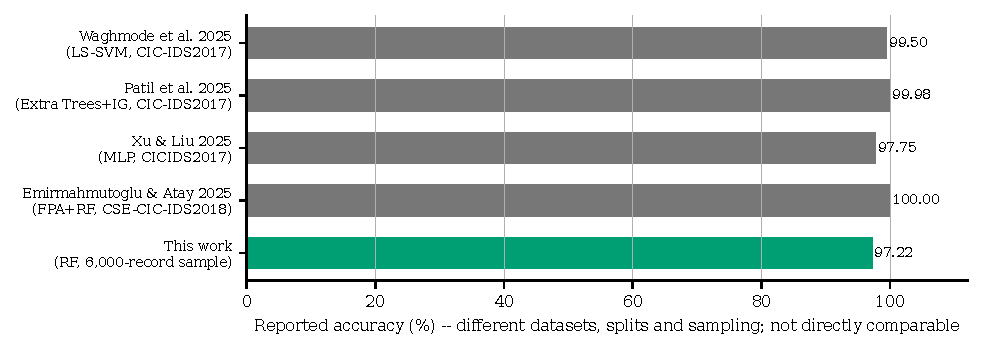
\includegraphics[width=0.85\textwidth]{figures/fig11_accuracy_comparison.pdf}
\caption{Accuracy reported by recent studies versus this work. Datasets, sampling, splits and metrics differ; the figure is not a performance ranking.}\label{fig:cmp}
\end{figure}

\section{Discussion}
\textbf{Answers to the research questions.} RQ1/RQ2: reducing 78 standardised features to 5--30 PCA or KPCA components generally did not improve and usually lowered macro-F1: clearly for decision tree and random forest, negligibly for logistic regression (30 components) and $k$-NN; the one gain, RBF-SVM with cosine KPCA, largely disappeared under tuning (0.076 to 0.021). RQ3: for $k$-NN, DT and RF the kernel mattered slightly more than component count, for LR and SVM the reverse; default-$\gamma$ RBF was weakest for four of five classifiers, and linear KPCA equals PCA. RQ4: KPCA multiplied reducer fit time by more than 200 and traced memory by about 37 at $n=4{,}800$ (quadratic in memory) with no benefit for four of five classifiers. RQ5: orderings were stable across repeated folds, training sizes, nested selection, tuning, and the scorable row-order splits.

\textbf{Why accuracy misleads.} The benign class is 67.2\,\% of records, so the trivial baseline already has accuracy 0.672. The best model's accuracy of 0.972 corresponds to macro-F1 0.901 and web-attack F1 values of 0.53 and 0.59: a systematic failure on two classes that accuracy cannot reveal, nor whether a one-point difference is noise (fold standard deviations of macro-F1 are 0.02).

\textbf{Untested explanations.} Tree ensembles are scale-insensitive, and a few leading components may discard discriminative low-variance directions; untested.

\section{Threats to Validity and Limitations}
These limitations are real, and the conclusions should be read as conditional on them.

\textbf{1. Sample, not full data.} All results come from \emph{one} stratified sample of 6{,}000 records out of 2.5\,M de-duplicated flows (0.24\,\%), because exact KPCA is quadratic in memory. The sample has a floor of 100 records per class and is \emph{not} prevalence-preserving: attack classes are over-represented, so accuracy, macro-F1 and class priors do not describe deployment-time prevalence. Heartbleed (11 records), SQL injection (21) and infiltration (36) are complete but tiny, so their per-class estimates are very uncertain, and another random sample could change rankings that differ by a few points. We did not repeat the pipeline over several sampling seeds.

\textbf{2. Leakage status.} Sampling was performed on the raw, un-imputed data, and imputation, scaling and reduction are fitted inside each training fold. Remaining possible leakage channels were \emph{not} eliminated: records from the same attack session or burst can still fall into both training and test folds in the random 5-fold design, and near-duplicate (not exact-duplicate) flows are not removed. The row-order checks reduce but do not remove this concern, and they rest on the unproven assumption that row order follows capture time.

\textbf{3. Limited external validity.} All data come from one dataset captured in one testbed over one week. The row-order checks score only seven classes (head/tail split) or six to ten classes per fold (blocked) and use a single split or five folds; there is no cross-dataset evaluation. The conclusions apply to random and within-file row-ordered splits of CIC-IDS2017 only; they say nothing about true temporal drift.

\textbf{4. Selection and inference.} The headline configuration (RF, original features) was the best of 189 on the same cross-validation that produced its score. The nested analysis shows the optimism is about 0.001 macro-F1 here, but the nested estimate itself is conditioned on the same sample. Repeated-CV significance tests violate independence \cite{nadeau2003}; $p$-values are screening evidence, and unadjusted values are reported for the nested comparisons.

\textbf{5. Limited tuning.} Hyper-parameter search covered only $k$-NN, SVM and random forest, four spaces and five outer folds, with small grids whose optimum lay on the edge for $k$-NN and SVM $C$. Logistic regression, the decision tree and the KPCA kernel parameters ($\gamma$ for RBF) were not tuned, so conclusions about those are about default settings. Class weighting was the only imbalance treatment; resampling was not evaluated.

\textbf{6. Dataset quality and cost.} The original CIC-IDS2017 flows contain known labelling and feature-construction artefacts \cite{engelen2021}, which may distort scores (and may explain the web brute-force/XSS confusion); we did not use the corrected release. Timings and memory come from one 2-vCPU virtual machine, memory is a traced lower bound, and the 64\,TB figure is arithmetic, not a measurement.



This study proposes no new algorithm, and we make no claim of state-of-the-art, real-time, production-ready or generalizable performance. The supported finding is narrower: on this sample, original features were at least as good as PCA or KPCA for four of five classifiers, the one exception largely vanished with tuning, and accuracy hid a systematic failure on web attacks.

\section{Conclusion}
On a 6{,}000-record sample drawn after exact same-label duplicate removal from all eight CIC-IDS2017 files, with fold-wise fitting of imputation, scaling and reduction, a random forest on the original 78 features had the highest observed macro-F1 (0.901 $\pm$ 0.020; accuracy 0.972 $\pm$ 0.004; 0.900 $\pm$ 0.022 with nested selection). PCA and KPCA with 5--30 components generally did not improve on the original features: they were clearly worse for decision tree and random forest, practically equal for logistic regression (30 components) and $k$-NN, and helped mainly the RBF-SVM (cosine KPCA), an advantage that shrank from 0.076 to 0.021 after tuning. The ranking survived row-order checks that rest on an assumed row order. Linear KPCA coincided with PCA. KPCA cost more than 200 times more fit time and 37 times more traced memory at 4{,}800 records. Accuracy (0.972) concealed weak detection of web brute force and XSS (F1 0.53, 0.59). The results are limited to this sample and to CIC-IDS2017.

\textbf{Future work.} Repeat the pipeline over several sampling seeds and larger samples with an approximate KPCA; add cross-dataset evaluation; widen the tuning grids and tune the KPCA kernel parameters; test the corrected CIC-IDS2017 release \cite{engelen2021}; and evaluate session-grouped splits.


\section*{Data and Code Availability}
The raw CIC-IDS2017 MachineLearningCVE files are distributed by the dataset provider \cite{sharafaldin2018} and are not redistributed here. The sampling script, the sampling manifest (file names, raw and de-duplicated class counts, seed), all experiment, analysis and claim-checking code, per-fold raw results and the generated tables and figures are available at [REPOSITORY URL / ARCHIVE DOI - TO BE FILLED BY THE AUTHORS]; the file \texttt{RUN\_EXPERIMENTS.md} lists the commands.


\section*{Acknowledgments and AI-assistance disclosure}
\textbf{[THE AUTHORS MUST CONFIRM THAT THIS DISCLOSURE IS ACCURATE AND COMPLETE, AND ADD ANY OTHER TOOL USED, BEFORE SUBMISSION.]} Generative AI was used in this work: Claude (Anthropic; Claude Code, model Claude Sonnet 5.5) helped (i) write and revise the Python pipeline (data preparation, cross-validation, nested CV, tuning, row-order checks, statistics, runtime benchmark, tables, figures and an automated claim checker); (ii) draft and edit the text of all sections, including the abstract, captions and limitations; and (iii) look up and cross-check bibliographic metadata and statements attributed to cited sources. All reported numbers were produced by code run on the data described and re-checked by script. The authors reviewed the content and remain fully responsible for it. [FUNDING / ACKNOWLEDGMENTS -- TO BE FILLED BY THE AUTHORS.] The authors declare no competing interests [TO BE CONFIRMED BY THE AUTHORS].

\bibliographystyle{splncs04}
\bibliography{references}
\end{document}
